\documentclass[10pt]{beamer}

\usepackage[UKenglish]{babel}
\usepackage{hyperref}
\usepackage[utf8]{inputenc}
\usepackage[backend=bibtex,style=ieee,maxbibnames=99]{biblatex}
\usepackage[uni,footuni,headframelogo]{./unirostock/beamerthemeRostock}
\usepackage{scrhack} %Fix for older packages

\title{IuK-Blockchain}
\subtitle{Progress report}
\author{\textsc{Robert Kohlen}\newline\textsc{Richard Dabels}\newline\textsc{Maximilian Jung}\newline\textsc{Daniel Decker}\newline\textsc{Nis Meinert}}
\date{03.06.2018}
\footinstitute{Institut für Informatik}

\addbibresource{./references.bib}

\begin{document}

\begin{frame}
	\titlepage
\end{frame}

\begin{frame}{Task}
	\begin{itemize}
		\item Develop a private blockchain to use at the IuK chair
		\item Implement an example scenario:
		\begin{itemize}
			\item Validation of documents with the help of blockchains
		\end{itemize}
	\end{itemize}
\end{frame}

\begin{frame}{Requirements}
	\begin{itemize}
		\item Fast \& easy way for the user to validate documents
		\item Add/update/revoke documents (in form of checksums) on the blockchain
		\item Address on the blockchain represents the identity of the author
		\item Author can be validated by signing a message with the private key which belongs to his address
		\item Authentication of authors is harder and only possible via side-channel
	\end{itemize}
\end{frame}

\begin{frame}{Platform}
	\begin{itemize}
		\item Node software: Parity (Ethereum)
		\item Web interface: HTML5 + CSS3 + web3.js (Javascript ethereum interface)
	\end{itemize}
	\begin{figure}
		
\includegraphics[width=0.5\textwidth]{images/parity-ethereum-logo.png}
	\end{figure}
\end{frame}

\begin{frame}{Parity}
	\begin{itemize}
		\item Implementation of the Ethereum Virtual Machine (EVM)
		\item Supports multiple consensus algorithms, e.g. Proof of Authority (PoA)
		\begin{itemize}
			\item Blocks can only be added by approved accounts (validators, i.e. trusted Universities)
		\end{itemize}
		\item Developed by 131 contributors on GitHub
		\item Testing environment: 3 PoA nodes in docker environment
		\item \url{https://github.com/paritytech/parity}
	\end{itemize}
\end{frame}

\begin{frame}{Functions of the smart contract}
	\begin{itemize}
		\item Mapping: author  $\rightarrow$ document(s)
		\item Storing documents as checksum (SHA-3 256 bit)
		\item Read-only validation function: Input checksum $\rightarrow$ Output author address
		\item Add/Update/Revoke documents
	\end{itemize}
\end{frame}

\begin{frame}{Interaction with the smart contract - web interface}
	\begin{itemize}
		\item Metamask (browser extension) for interaction with the blockchain
	\end{itemize}
	\begin{figure}
		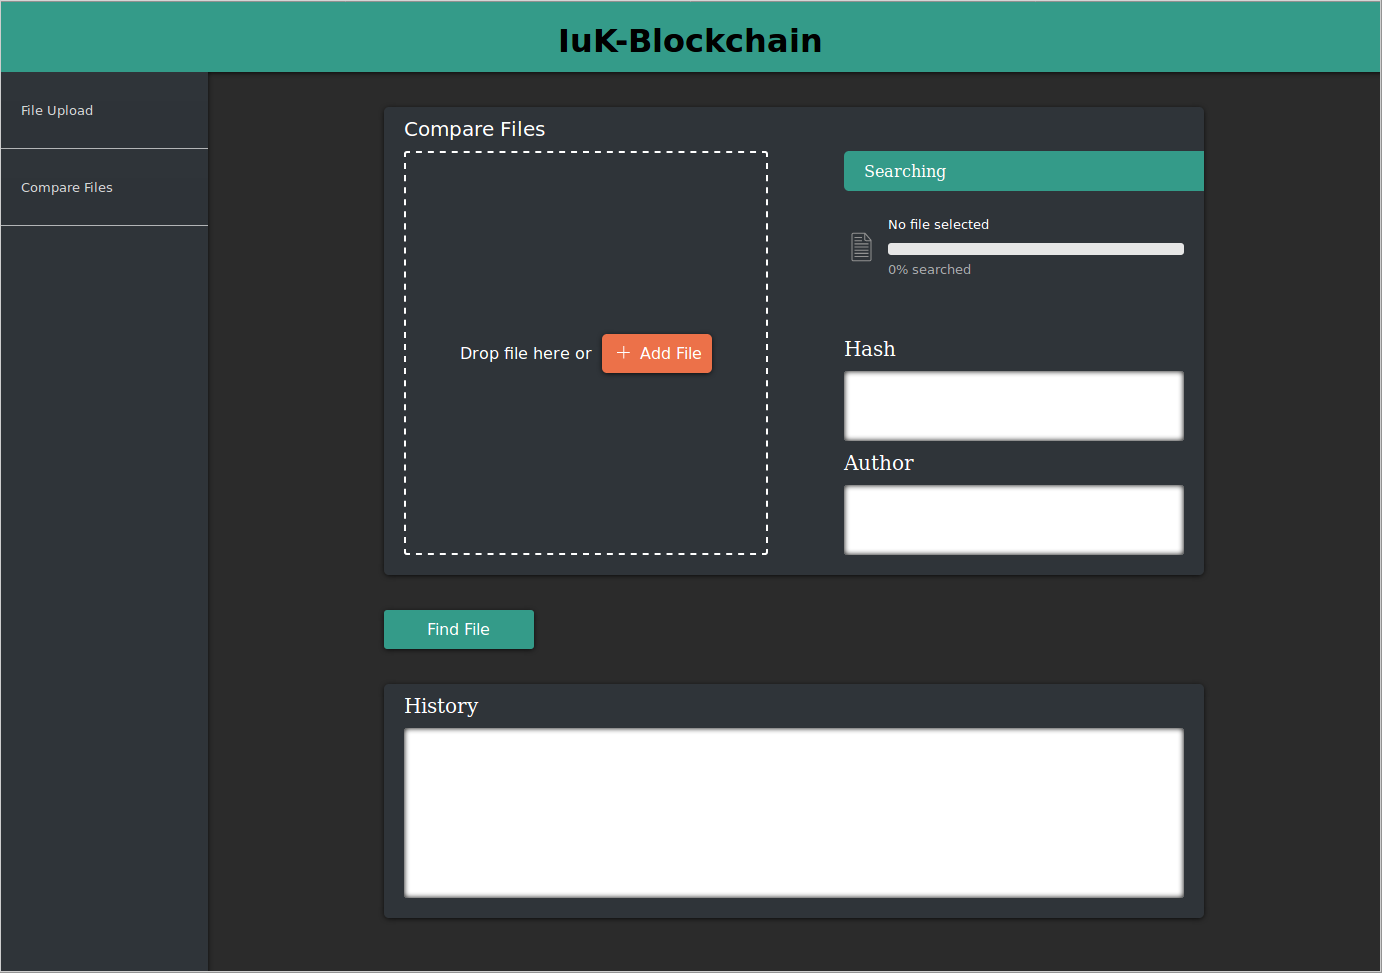
\includegraphics[width=0.78\textwidth]{images/GUI-180603_1.png}
	\end{figure}
\end{frame}

\begin{frame}{*Some* possible attack scenarios}
	\begin{itemize}
		\item Block document checksums by adding a large number of checksums
		\begin{itemize}
			\item Prevention: hash function with sufficient length, e.g. SHA256
			\item Pre-computation of possible checksums not plausible (One-Way-Function)
		\end{itemize}
		\item DDoS validator nodes to prevent interaction with the smart contract
		\begin{itemize}
			\item Prevention: Good firewall or fallback servers
		\end{itemize}
		\item Misbehaving/malicious validator nodes
		\begin{itemize}
			\item Countermeasure: Revoke validator rights
		\end{itemize}
	\end{itemize}
\end{frame}

\begin{frame}{Open questions}
	\begin{itemize}
		\item Should author of an document be changeable?
		\item Would an attacker free the document by himself?
	\end{itemize}
\end{frame}

%\begin{frame}[allowframebreaks]{References}
%Reduce URL font size
%\renewcommand{\UrlFont}{\small\rmfamily}
%\printbibliography
%\end{frame}

\end{document}
